\title{Manual de uso del editor de texto \texttt{Vim}}
\author{Gabriel López}
\date{\today}

\documentclass[10pt]{article}
\usepackage[spanish]{babel}
\usepackage{graphicx}
\usepackage[letterpaper]{geometry}


\begin{document}
\maketitle

\section{\texttt{Vim}, un editor de texto minimalista.}
\texttt{Vim} es un editor de texto creado por Brian Moolenaar. Es una versión mejorada del editor de texto \texttt{vi} creado por el programador Bill Joy. 
El editor de texto \texttt{Vim} es un editor de texto pensando para ser un programa de edición de texto minimalista y extensible, lo que significa que con ayuda de programas auxiliares hechos por la comunidad conocidos como \textit{plugins}, se puede utilizar el editor \texttt{Vim} como un entorno de programación (conocido como \textit{IDE}) o un entorno minimalista de edición de documentos hechos en \LaTeX. \\ 
Si bien, aprender a usar \texttt{Vim} es un proyecto con un curva de aprendizaje un poco pronunciada, este editor ofrece ciertas ventajas por sobre otros editores, sobre todo a nivel de personalización, configuración y uso de recursos, lo que lo hace ídoneo en \textit{hardware} de capacidad limitada. 
Además de esto, con la correcta configuración y el correcto uso de \textit{plugins}, la escritura (sobre todo de documentos de tipo científico) puede ser más fluida a un nivel muy similar a la toma de notas manuscritas. 
\section{Entornos en \texttt{Vim}}
\texttt{Vim} es un editor de texto poco ortodoxo comparado con el resto de los editores de texto que están disponibles para uso público, para empezar, \texttt{Vim} usa un esquema de entornos \textit{entornos}, lo que quiere decir, que para las acciones que usualmente se ven relegadas al uso del ratón en otros editores, en \texttt{Vim} están relegadas a un \textit{entorno}. Los entornos de uso básico son los siguientes:
\begin{itemize}
	\item \textit{NORMAL}: Este entorno es el entorno básico de \texttt{Vim}. En este entorno se utiliza para navegar entre líneas de texto, borrar contenido y introducir comandos dentro del editor.
	      La utilidad del modo \textit{NORMAL} radica en el uso de comandos para usar la terminal y el editor al mismo tiempo. 
	\item \textit{INSERTAR}: Este entorno se utiliza para la inserción de texto dentro de líneas en el editor. Para entrar a este entonro basta con introducir la tecla \texttt{i} mediante el teclado.
Una vez que la tecla se ha introducido, el editor colocará el texto \texttt{INSERTAR} o \texttt{INSERT} en la parte inferior de la pantalla, denoatando que el modo de inserción está activado. 
	\item \textit{VISUAL}: Este entorno se encarga de función de copiar y pegar contenido de las lineas. Para entrar a este modo, se debe introducir \texttt{v} con el teclado.
Una vez que el modo \textit{VISUAL} está activado debe aparecer en pantalla la leyenda \texttt{VISUAL} en la esquina inferior izquierda. 
\end{itemize}
Es importante destacar que para salir de un entorno para entrar de nuevo al entorno \textit{NORMAL} se introduce la tecla \texttt{Esc} con el teclado. Para ilustrar los entornos de \texttt{Vim} colocamos la siguiente imagen. En dicha imagen es notorio que debido al idioma con el que se tiene el ordenador, aparece la leyenda \texttt{INSERTAR} en la parte inferior, denotando que el modo de inserción de texto está activo. 
\begin{figure}[h]
	\centering
	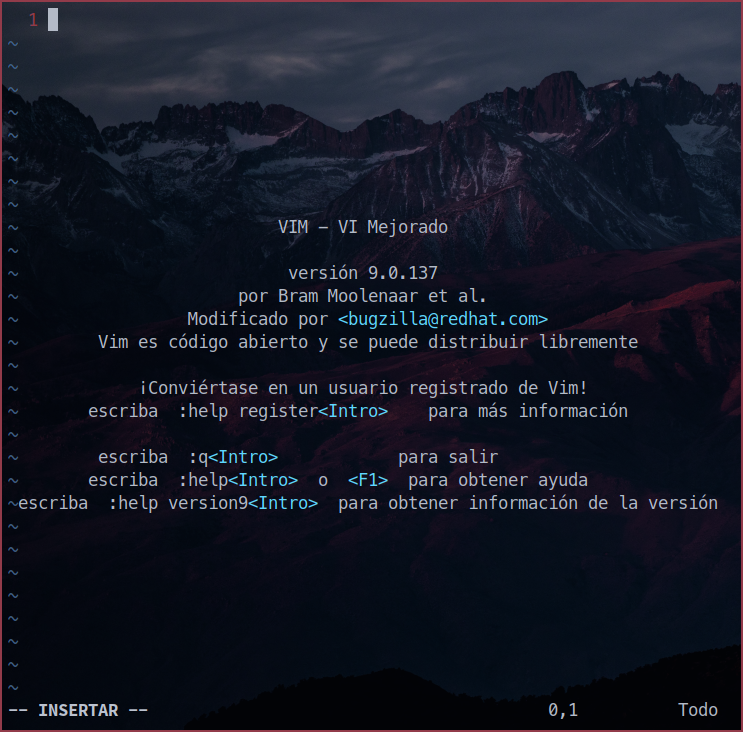
\includegraphics[scale=0.6]{./img/Vim_INS.png}
	\caption{\texttt{Vim} en el modo \textit{INSERTAR}}
\end{figure}
\newline
A pesar de todo esto, existen muchos más entornos dentro del editor, sin embargo, consideramos que estos tres son los más útiles para un usuario nuevo de \texttt{Vim} debido a que facilitan la escritura de documentos y permiten la introducción de comandos dentro del mismo. 
\newpage
\section{¿Cómo salir de \texttt{Vim}?}
Es normal que el usuario novato de GNU-Linux o cualquier sistema operativo derivado de UNIX. De modo que el sistema operativo a veces deja el usuario dentro de \texttt{Vim} sin ningún aviso de cómo salir del editor de texto. Por esta razón en esta sección se explicará como salir de \texttt{Vim}. \\
Para empezar, la imagen inicial que el usuario tiene al entrar a \texttt{Vim} es la siguiente: \newline
\begin{figure}[h]
	\centering
	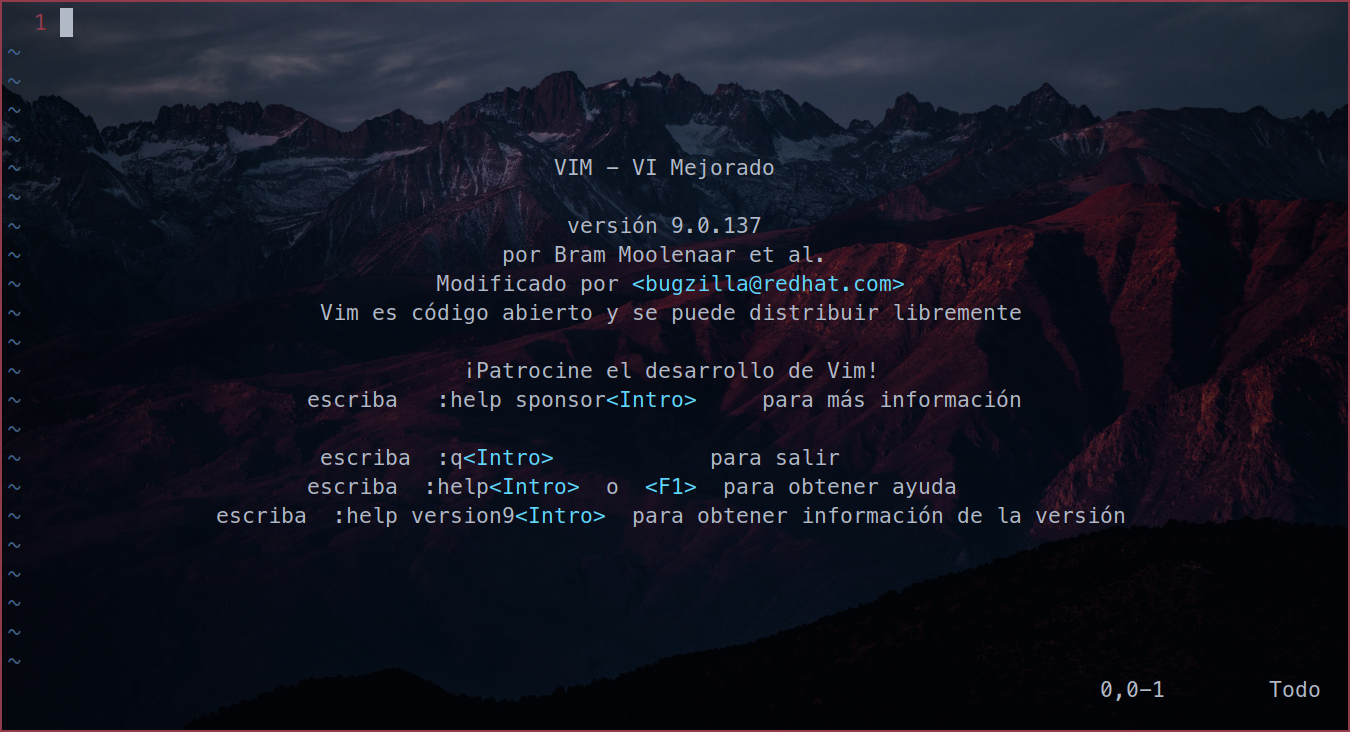
\includegraphics[scale=0.4]{./img/poisson_mu1.png}
	\caption{Primera impresión de \texttt{Vim}}
\end{figure}
\newline
Podría parecer que \texttt{Vim} es complicado, pero en realidad, salir del editor es relativamente sencillo, la secuencia de pasos para salir de \texttt{Vim} es la siguiente:
\begin{itemize}
	\item Primero, si usted desea guardar el contenido del archivo, es conveniente guardar el contenido del archivo primero, esto se logra mediante el comando \texttt{:w} dentro del entorno \textit{NORMAL}.
	\item Ahora que el archivo está guardado, es posible salir del editor sin problemas, por lo que se procede a colocar el comando \texttt{:q} dentro del mismo entorno \textit{NORMAL}.
\end{itemize}
Si bien es posible que queramos guardar el contenido de nuestro archivo de texto, también tenemos la opción de salir sin guardar (no recomendada a menos que se desee salir de \texttt{Vim} si se entró por error), en este caso, basta con introducir el comando \texttt{:q!} en el modo \textit{NORMAL} del editor.
\section{¿Existe alguna forma de aprender \texttt{Vim} mediante ejemplos?}
Si bien \texttt{Vim} es un editor de texto que puede parecer poco ortodoxo al principio, existen formas para aprender su uso de una forma interactiva mediante ejemplos. En el caso de \texttt{Vim} existe el complemento denominado \texttt{vimtutor}, que es un complemento de consola que suele estar instalado en cualquier máquina UNIX. En el caso de querer acceder a dicho complemento, basta con introducir el comando \texttt{vimtutor} dentro de la terminal de GNU-Linux o su equivalente en UNIX. 
\section{Navegación en \texttt{Vim}}
\texttt{Vim} es un editor de texto que tiene un esquema de navegación diferente al resto de editores de texto que podemos encontrar en el mercado. Esto es debido a cuestiones de convención. 
Si bien, las teclas direccionales del teclado funcionan para navegar entre texto dentro del editor, su uso no es recomendado por la mayoría de guias de uso de \texttt{Vim}. \\
\subsection{Navegación básica en \texttt{Vim}}
Esto se entiende mejor con los ejemplos proporcionados por el complemento de consola llamado \texttt{vimtutor}. Para nuestros efectos, se busca introducir al usuario a los conceptos básicos de los que \texttt{Vim} para que sea capaz de redactar documentos simples dentro del editor. Dicho esto, podemos mostrar el esquema básico de navegación del que hace uso \texttt{Vim}.
\begin{figure}[h]
	\centering
	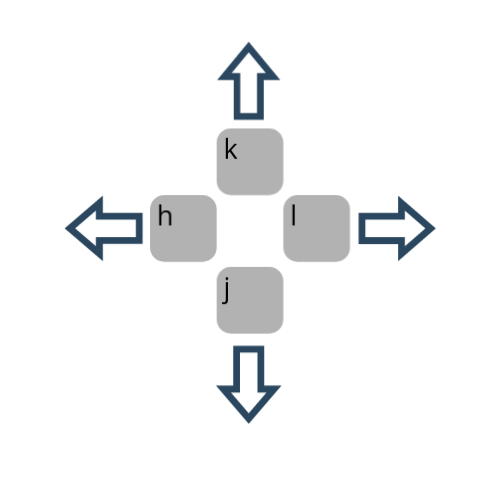
\includegraphics[scale=0.3]{./img/vim_nav.png}
	\caption{Esquema de navegación básico dentro de \texttt{Vim}}
\end{figure}
\newline
Para resumir, podemos ver que las teclas de navegación son las siguientes:
\begin{itemize}
	\item \texttt{k} y \texttt{j} son usadas para subir y bajar de linea, respectivamente. 
	\item \texttt{h} y \texttt{l} son usadas para desplazarse de izquierda a derecha, respectivamente. 
\end{itemize}
Como se puede ver, el esquema de navegación dista de los editores convencionales. Esto es por diseño, ya que  \texttt{Vim} hace uso de estas mecánicas de movimiento para tratar dicho movimiento como si fuera un \textit{comando de consola} y esto permite aplicar ciertos comandos, como el de \textit{borrar} al movimiento para alcanzar cierta velocidad a la hora de borrar contenido dentro de una línea de texto. 
\newpage
\subsection{Otras opciones de movimiento en \texttt{Vim}}
Como se mencionó anteriormente, \texttt{Vim} trata el movimiento como si fuera un comando de consola, esto permite aplicar ciertos efectos al movimiento.
Si bien, el movimiento básico se resume con las teclas, \texttt{h,j,k} y \texttt{l}, existen también cuatro comandos útiles que deben ser mostrados para que este manual se pueda considerar una referencia útil para el uso de \texttt{Vim}.
En general, \texttt{Vim} suele trabajar por \textit{palabras}cuando se habla de navegación dentro de una linea de texto, entonces existen formas para desplazarse en una linea de texto de palabra en palabra. En este caso, existen cuatro comandos destinados para esta función:
\begin{itemize}
	\item El comando \texttt{w} permite al usuario desplazarse desde su localización actual hacia el \textit{inicio} de la siguiente palabra en la linea de texto. 
	\item El comando \texttt{e} permite al usuario desplazarse desde su actual ubicación, hacia el \textit{final} de la siguiente palabra en la linea actual de texto.
	\item Se usa el número \texttt{0} para desplazarse hacia el \textit{inicio} de la linea.
	\item Finalmente, el comando \texttt{\$} se usa para desplazarse hacia el \textit{final} de la linea.
\end{itemize}
\section{La función de \textit{Borrar} en \texttt{Vim}}
Como cualquier editor de texto plano, usualmente queremos editar el contenido de nuestro archivo, ya sea cambiando algunas lineas dentro del archivo o \textit{borrando} contenido dentro de las líneas. En \texttt{Vim} la función de \textit{borrar} dentro del documento está relativamente ligada al uso de movimiento.\\
Esto es debido a que podemos pensar en lo siguiente: la función de borrar se activa con el comando \texttt{d} y la cantidad de contenido a borrar se determina usando los comandos de movimiento vistos anteriormente. Por lo que, para ilustrar algunos de los usos de este mecánica, es conveniente colocar algunos de los comandos más utilizados con esta modalidad. 
\begin{itemize}
	\item El comando \texttt{dw} permite borrar todo lo que está desde \textit{la ubicación actual hasta el inicio de la siguiente palabra.} Como ven, el comando de \textit{borrar} se antepone a la opción de movimiento.
	\item Introduciendo \texttt{de} podemos borrar todo aquello que está comprendido desde \textit{la localización del puntero en el editor, hasta el final de la siguiente palabra en la linea}. 
\end{itemize}
Como podemos observar, el comando de \textit{borrar} en \texttt{Vim} usualmente está antes de la opción de movimiento. Sin embargo, debido a razones que los creadores de \texttt{Vim} comentan en \texttt{vimtutor} es común que se requiera \textit{borrar una o más lineas completas}. \\
En este caso, la función de borrar es mucho más sencilla, solamente basta con introducir el comando \texttt{dd}. Es en este punto en donde es conveniente introducir una figura que está presente también en \texttt{Vim} y que al día de hoy, no hemos visto en otros editores de texto y que, al día de hoy, no hemos visto en otros editores de texto, esta característica se conoce como \textit{contadores}.
\subsection{Contadores}
Los \textit{contadores} son una característica de \texttt{Vim} que permite al usuario repetir un comando un determinado número de veces, usualmente \texttt{vimtutor} relega la lección de esta característica hasta que ya se han visto los comandos básicos de movimiento y borrado y en este caso, es conveniente explicar un poco el porqué. Supongamos lo siguiente: Se desea borrar un número determinado de líneas en el editor, si se usaran otros editores, se podría pensar en usar el ratón para seleccionar las líneas y borrarlas con la tecla \texttt{backspace}.\\
Sin embargo, en \texttt{Vim} se debe aplicar el uso de los comandos vistos anteriormente. Un ejemplo simple sería el borrado de 4 lineas en un archivo de texto. En este caso, el comando a utilizar es: \texttt{4dd}. La explicación del comando es la siguiente: 
\begin{itemize}
	\item \texttt{4} es el número de veces que se repetirá el siguiente comando. 
	\item \texttt{dd} es el comando usado para borrar una linea completa en el documento de texto. 
\end{itemize}
Este es el uso más sencillo de los contadores en \texttt{Vim}, sin embargo, su uso no se limita solamente a esto, y es recomandable revisar la sección de contadores en el complemento \texttt{vimtutor} para una mejor comprensión del uso de esta característica del editor. 
\end{document}

